%=============================================================================
% ..... THIS IS chapter{FREQRESP: ITU-T frequency response measure tool } .....
%
% ... Authors (STL2005):  Cyril Guillaum� & St�phane Ragot - 
% ... revised (STL2009) by Yusuke Hiwasaki (NTT), Herve Taddei (Huawei), Claude Lamblin (France Telecom, Orange) - 
%
%=============================================================================
\chapter{ITU-T frequency response measurement tool}
%=============================================================================

%----------------------------------------------------------------------
\section{Introduction}
%----------------------------------------------------------------------

In order to measure effective codec bandwidth, a frequency response 
measurement tool was created for the STL2005 \cite{STL2005}. At Q10/16 January 2008 
meeting, a window overlap option was proposed to make this tool more 
accurate when dealing with signals with quickly varying frequencies 
while allowing the tool to be used as before \cite{AC-0801-Q10-31} and it was wondered whether this window overlap option should be the default mode. At this January 2008 meeting \cite{TD297R1}, it was also suggested that an option to use other window sizes might be useful. In addition, during G.729.1 Superwideband qualification phase, it was found that the speed of the algorithm can be sometime a bit too slow. Therefore, at Q10/16 September 2008 meeting, an update was provided to allow variable frame size usage and to increase the computation speed \cite{AC-0809-Q10-35}. 
In STL2009, the frequency response measurement tool has been revised to introduce these three options: window overlap, variable frame size, and increased computation speed. 
%----------------------------------------------------------------------
\section{Description of the algorithm}
%----------------------------------------------------------------------

An input signal is encoded and decoded by the Codec under Test. The
periodogram method is then used to compute the average amplitude
spectrum difference between a reference signal (e.g. the input file to
the speech codec) and a test signal (e.g. the speech signal after
encoding and decoding by a codec).

The input and output signals can be treated on a frame by frame basis,
with size power of 2 which defaults to 2048 if unspecified. A Hanning
window is applied to each input and output frame. The resulting
windowed signals are transformed to the frequency domain using a
various number of point Fast Fourier transform. The input and output
amplitude spectra are then computed and averaged. This tool produces
the average amplitude spectrum in ASCII and also produces a bitmap
file.

\subsection{Discrete Fourier Transform (DFT)}

The spectrum is computed using the Discrete Fourier Transform (for
real signals). This is performed as follows :
\[
    X(f)=\sum^{NFFT-1}_{k=0}x(k)\cdot \cos{(2\pi fk)} - j\cdot \sum^{NFFT-1}_{k=0}x(k)\cdot \sin{(2\pi fk)}
\]
where \emph{NFFT} is the number of DFT coefficients.
\subsection{Hanning window generation (DFT)}

The Hanning window of length n is defined as :
\[
    hanning(k)=0.5\cdot [1-\cos(2\pi \cdot \frac{k+1}{n+1})] \mbox{\rule{15mm}{0mm}} (0 \le k \le n-1)
\]

\subsection{Window overlap}

In STL2005, the frequency measurement tool used non-overlapping
windowed frames to perform the signal analysis. With such
non-overlapping Hanning windows, some regions of the signal are set to
a very weak value at the window edges. Thus some temporal parts of the
signal are not taken into account when applying the Fourier transform,
and are not visible in the frequency representation. This is a problem
when signals with very quick frequency changes, or continuous changes
are considered.  This case occurred with the sweep tone signal used in
G.722.1 fullband qualification phase. To fix this, an option has been
added to the tool to introduce overlapping between two consecutive
frames.  With this option, a temporal region attenuated by the Hanning
window in one frame will be present in next frame.  The desired
percentage of overlapping can be chosen. If the option is not
activated, the tool output remains unchanged.

\subsection{Variable frame size}
In STL2005, the window size used for discrete Fourier transform was
fixed to 2048 samples and could not provide changes in the frequency
resolution. In order provide more freedom, a variable window size was
implemented using Fast Fourier Transform (FFT) algorithm. The use of
FFT implies that the window size is a power of 2, thus, available
sizes are: 16, 32, 64, 128, 256, 512, 1024, 2048, 4096 and 8192. The
dimensions of the bitmap file created by the tool (with option
``-bmp'') are adapted to the new variable size: if the size is smaller
than 2048, then the bitmap file is in the same dimensions as for a
2048-sample bitmap file, because smaller dimensions would give
unreadable figures. For windows sizes larger than 2048, the bitmap
dimensions are increased to adapt to better frequency resolution.

The figures \ref{fig:femaleVoice256}, \ref{fig:femaleVoice2048},
\ref{fig:femaleVoice8192} give the bitmap files obtained with {\tt
  freqresp} tool operating in 256-, 2048- and 8192-sample windowing,
respectively. The input file was the artificial female voice
standardized by ITU in \cite{P.50}.

\newpage

%------------------------------------------------------------------------
\begin{figure}[!hbp]
  \begin{center}
    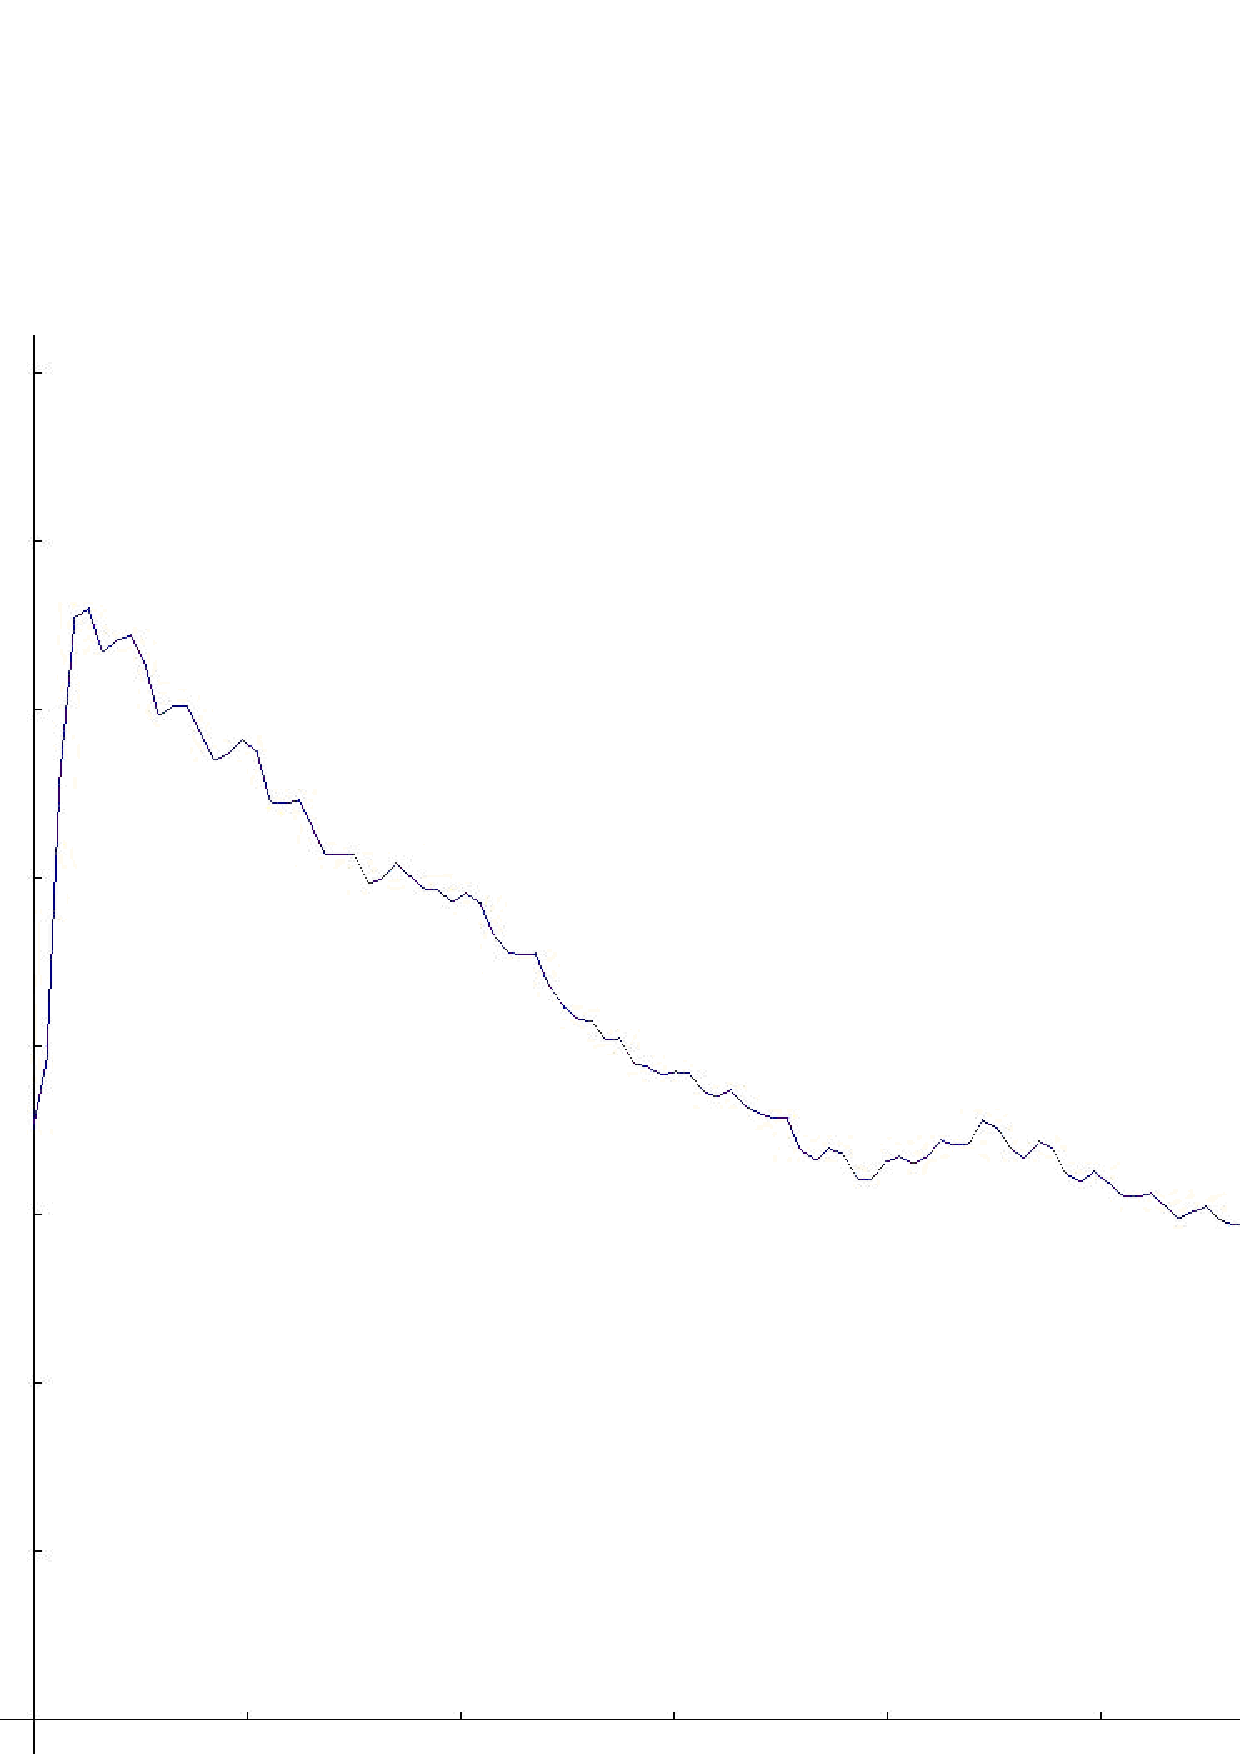
\includegraphics[scale=0.25]{femaleVoice256}
  	\caption{P.50 female voice analyzed with a 256-sample window\label{fig:femaleVoice256}}
  \end{center}
\end{figure}
\begin{figure}[!hbp]
  \begin{center}
    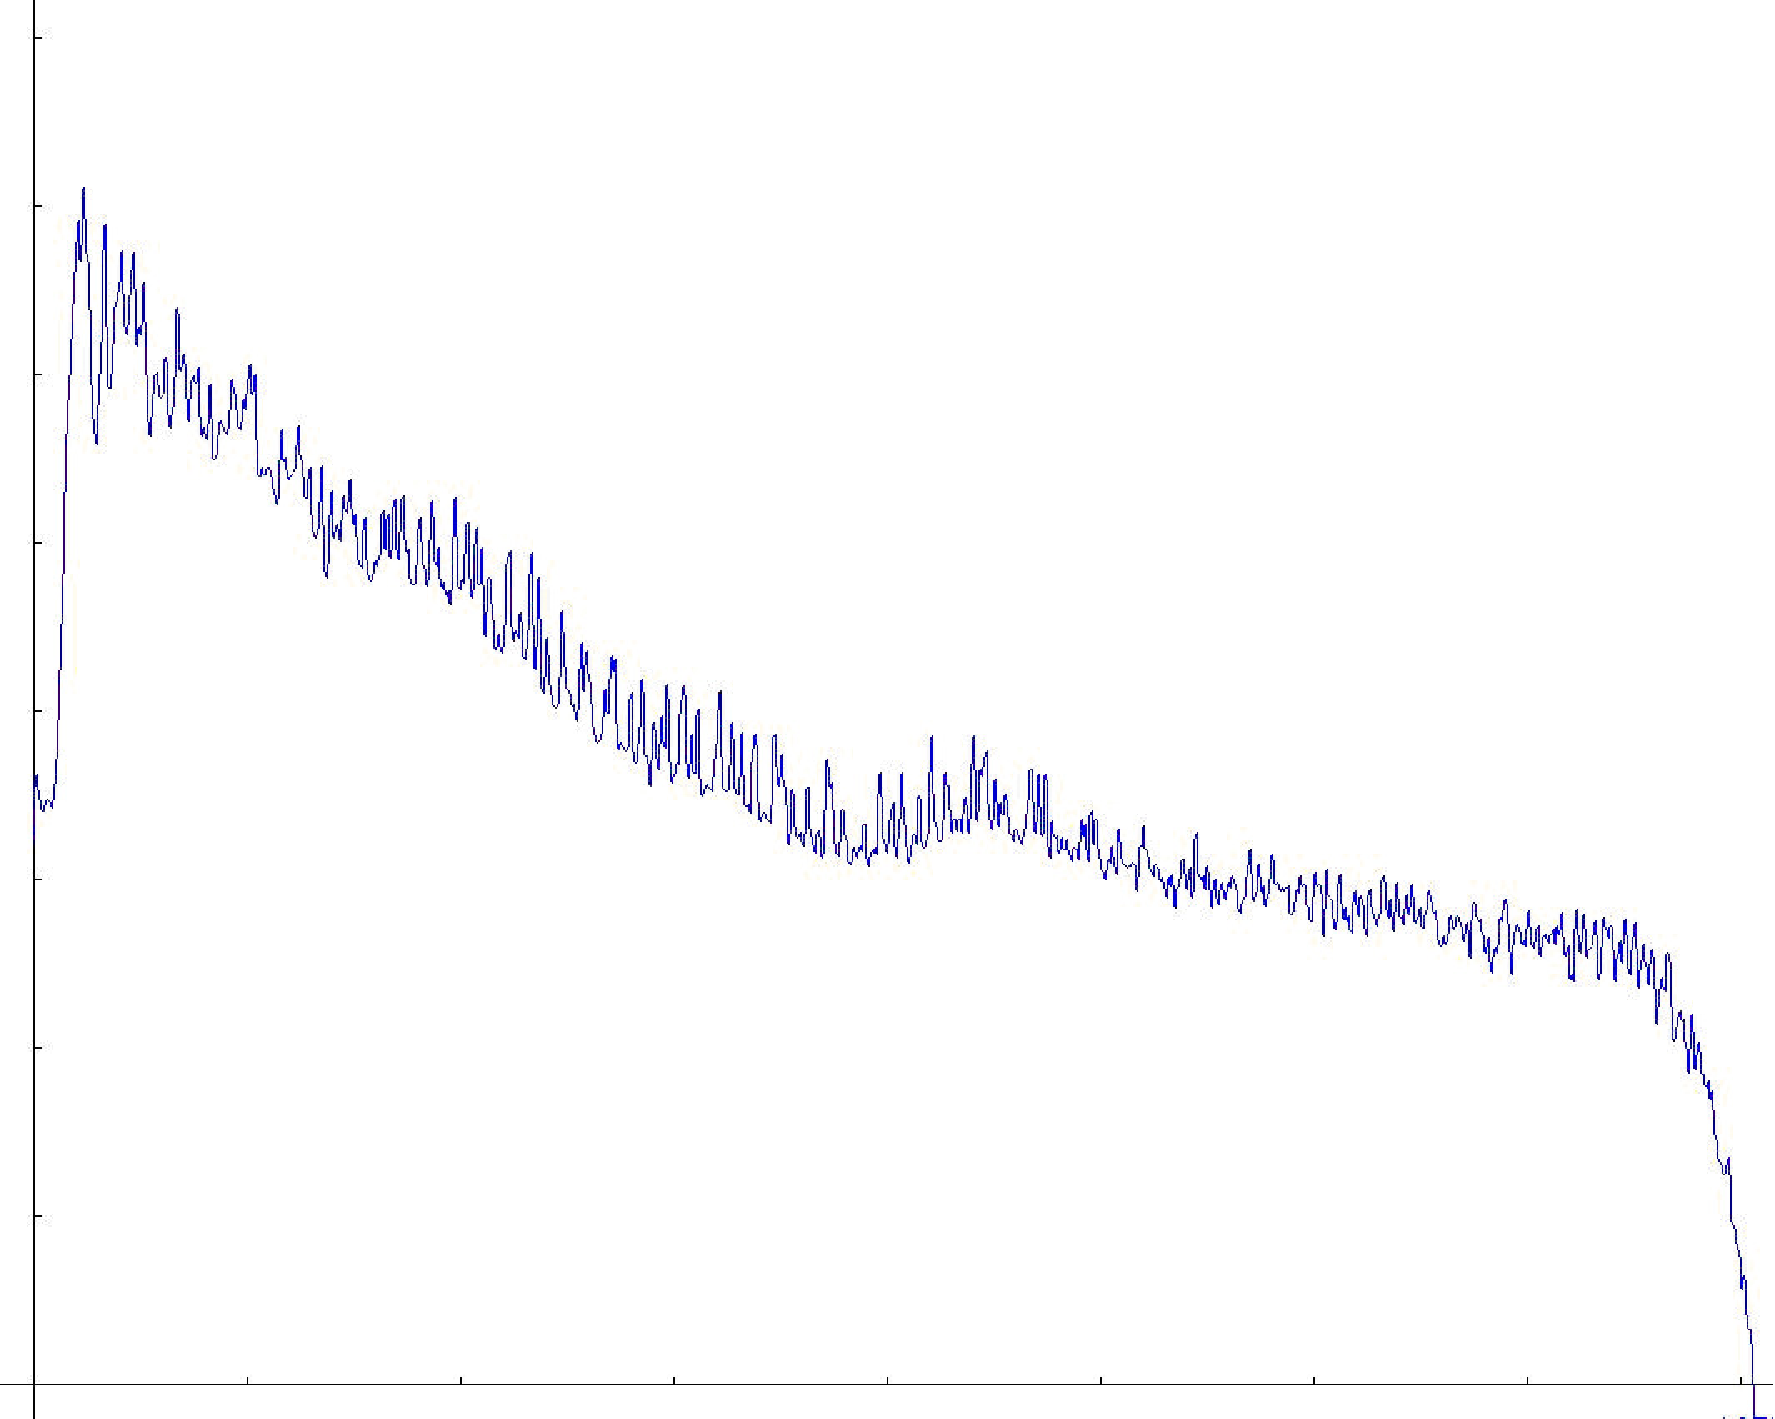
\includegraphics[scale=0.25]{femaleVoice2048}
  	\caption{P.50 female voice analyzed with a 2048-sample window\label{fig:femaleVoice2048}}
  \end{center}
\end{figure}
\begin{figure}[!hbp]
  \begin{center}
    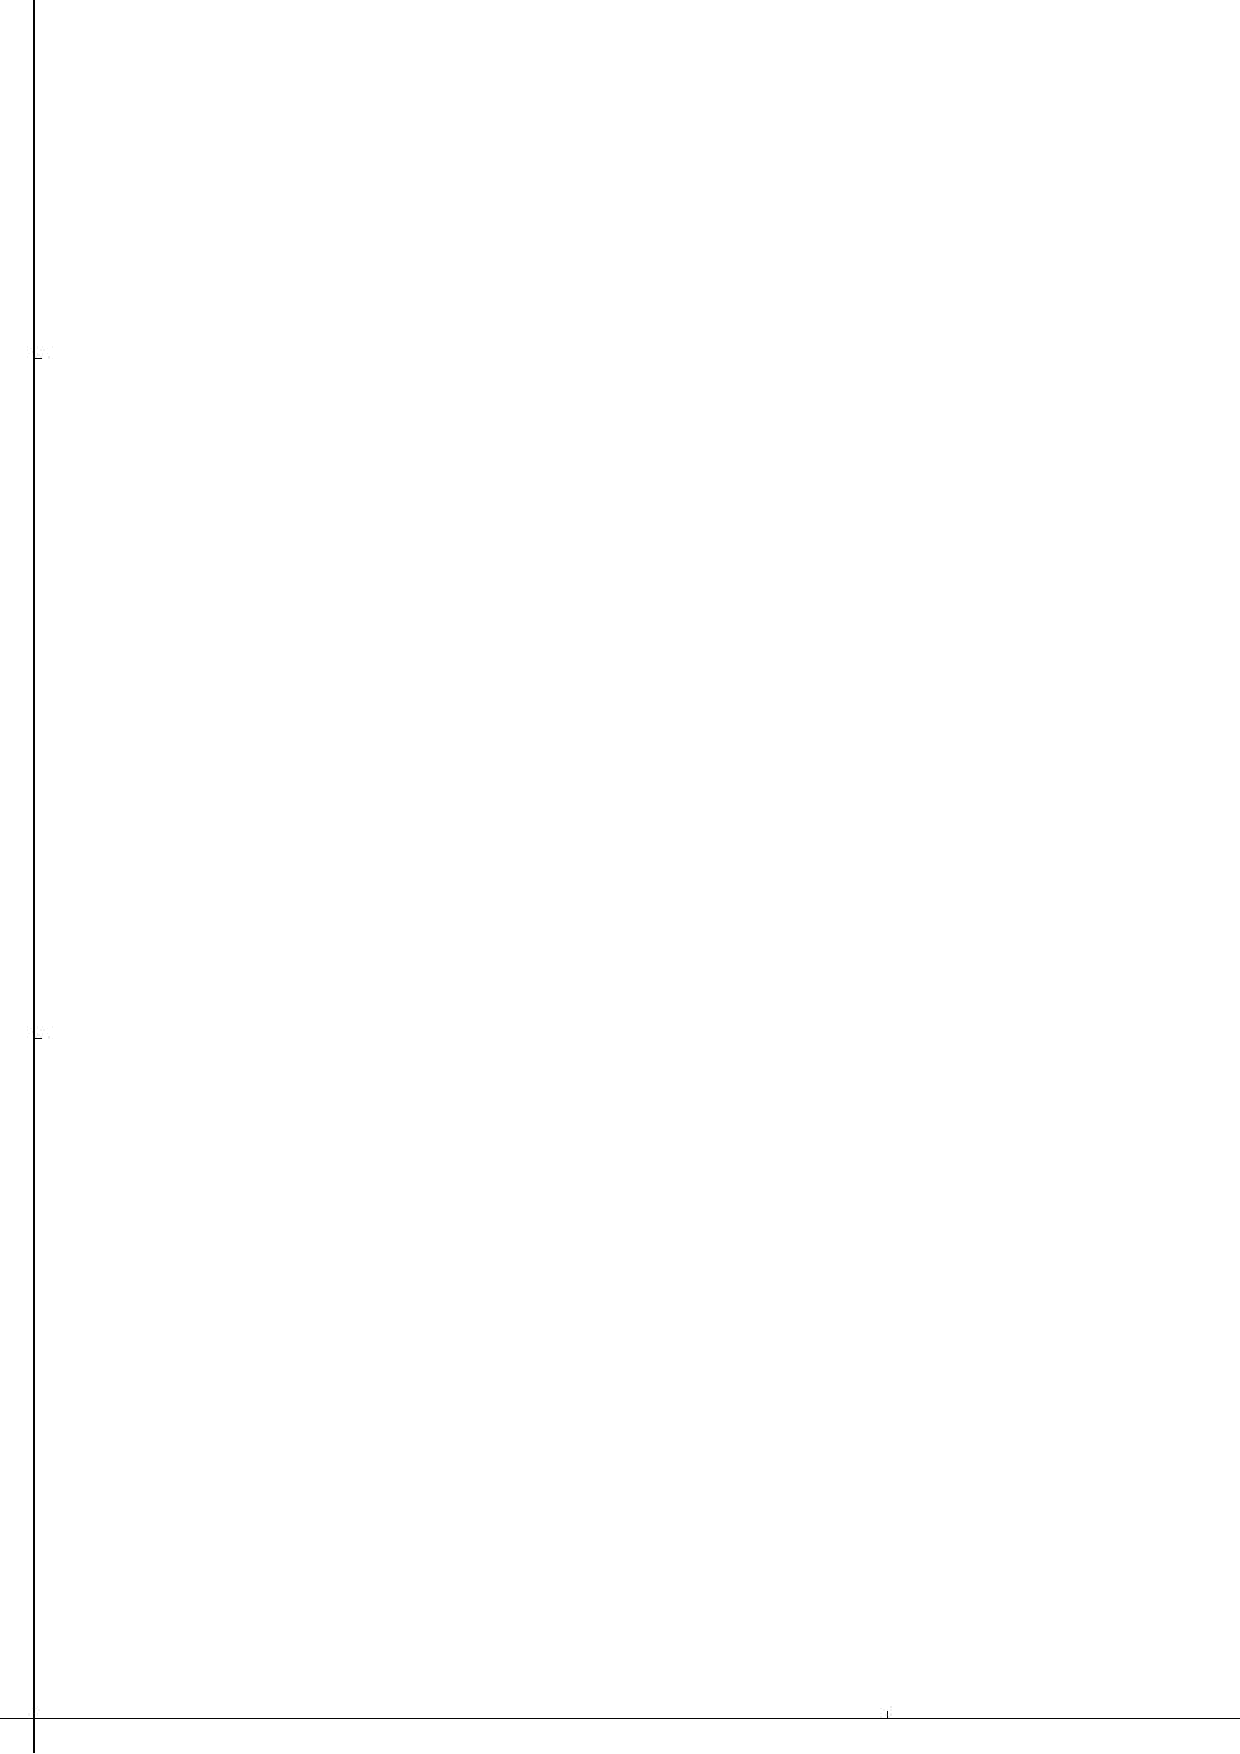
\includegraphics[scale=0.065]{femaleVoice8192}
	  \caption{P.50 female voice analyzed with a 8192-sample window\label{fig:femaleVoice8192}}
  \end{center}
\end{figure}
%------------------ End of figure ----------------------------------

\subsection{Computation optimization}

As the time needed for computing the frequency response of a long audio file can be rather long, the Discrete Fourier Transform (DFT) can be replaced by a split radix (4,2) Fast Fourier Transform (FFT) algorithm \footnote{Split-radix FFT algorithm, http:\/\/en.wikipedia.org\/wiki\/Split-radix\_FFT\_algorithm}.\\
When this option is activated the frame size is limited to power of 2 values (16-32-64-128-256-512-1024-2048-4096-8192).\\
%------------------------------------------------------------------------
% \begin{figure}[!hbp]
%   \begin{center}
%     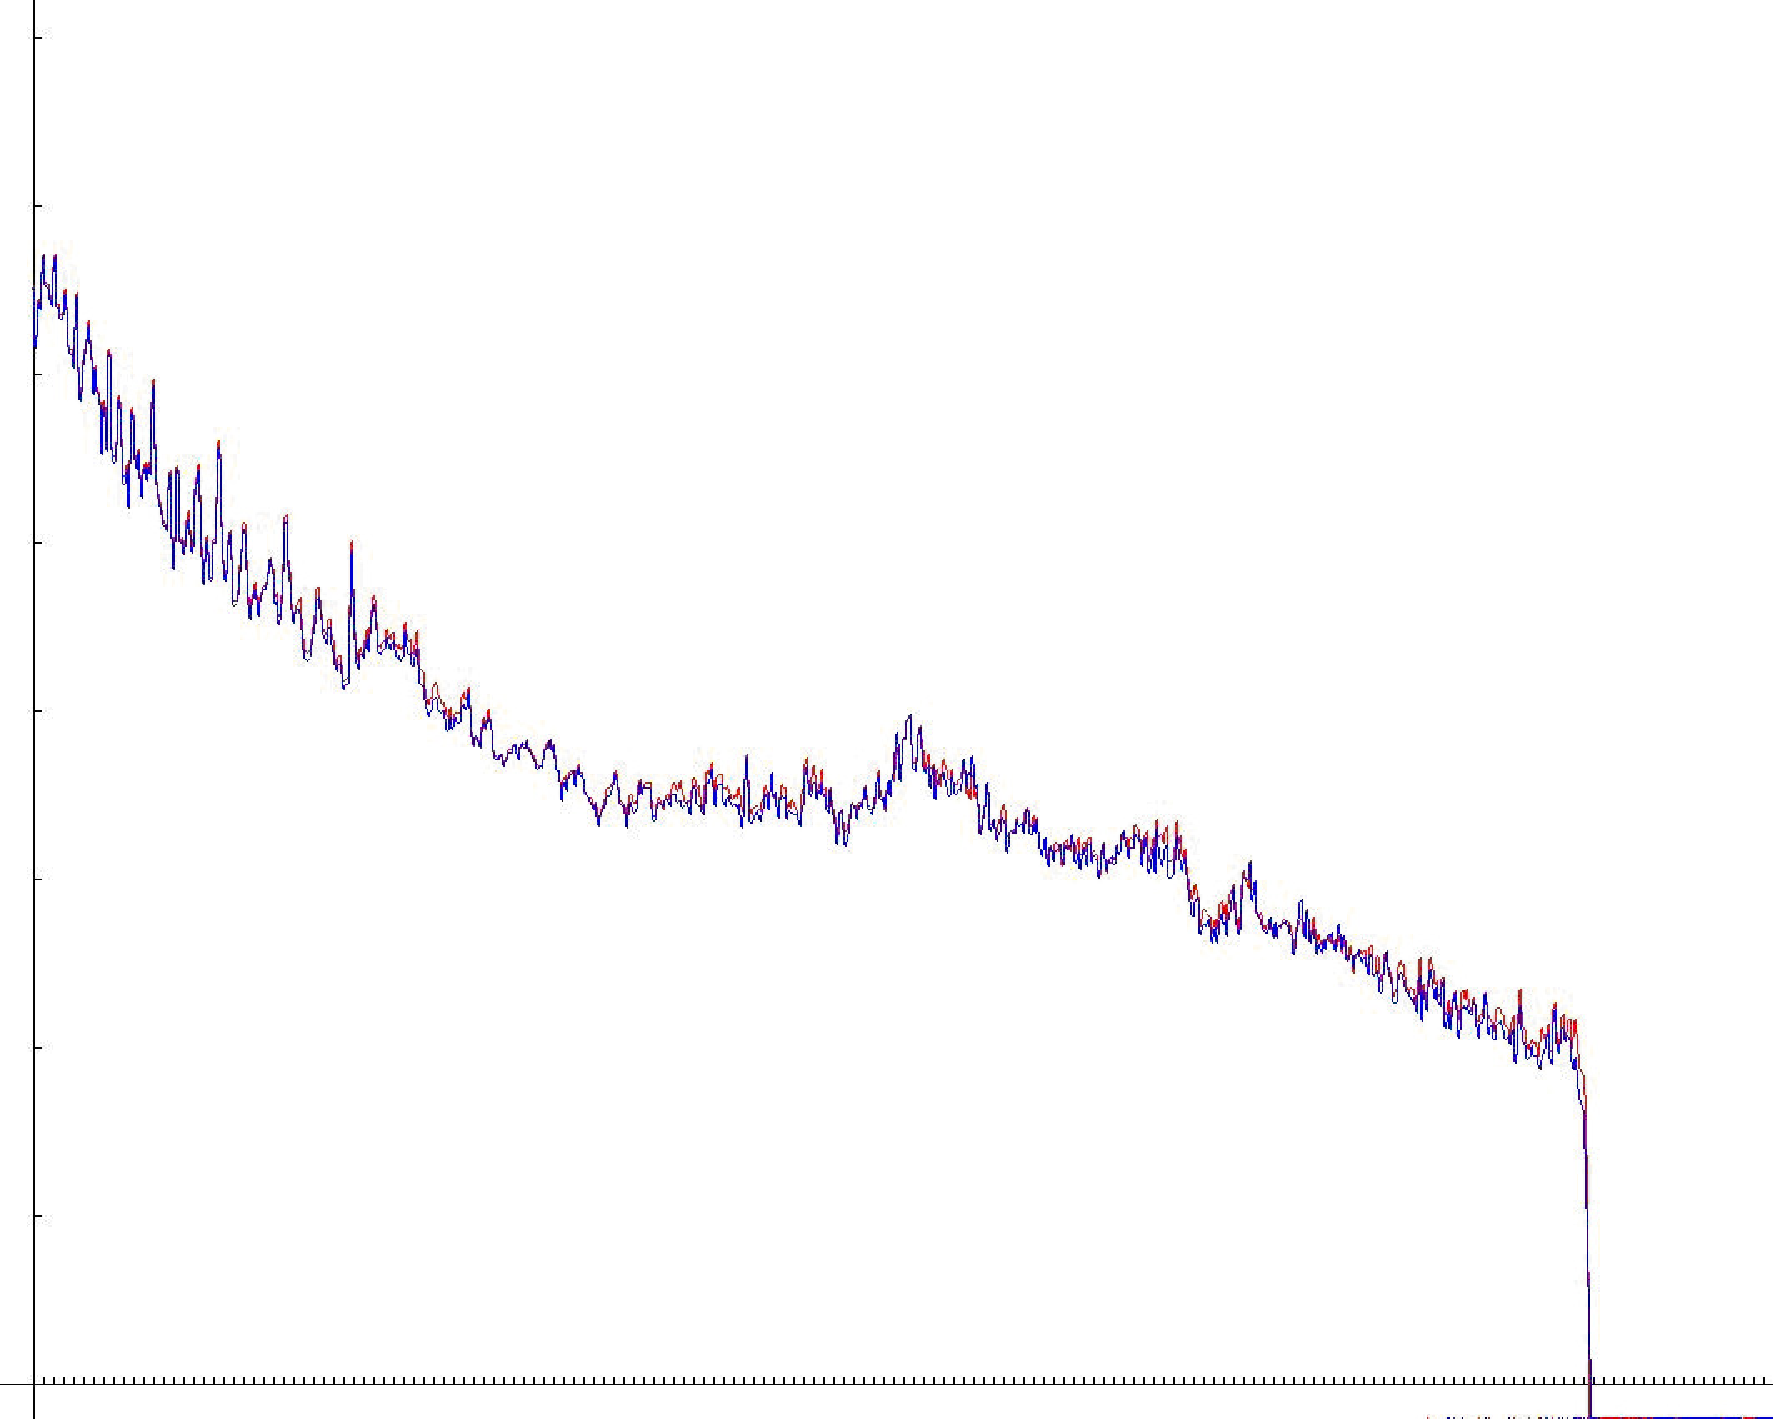
\includegraphics[scale=0.35]{withoutTUNEDFFT}
%   	\caption{When TUNED\_FFT is not activated the following frequency response is obtained:\label{withoutTUNEDFFT}}
%   \end{center}
% \end{figure}
% \begin{figure}[!htp]
%   \begin{center}
%     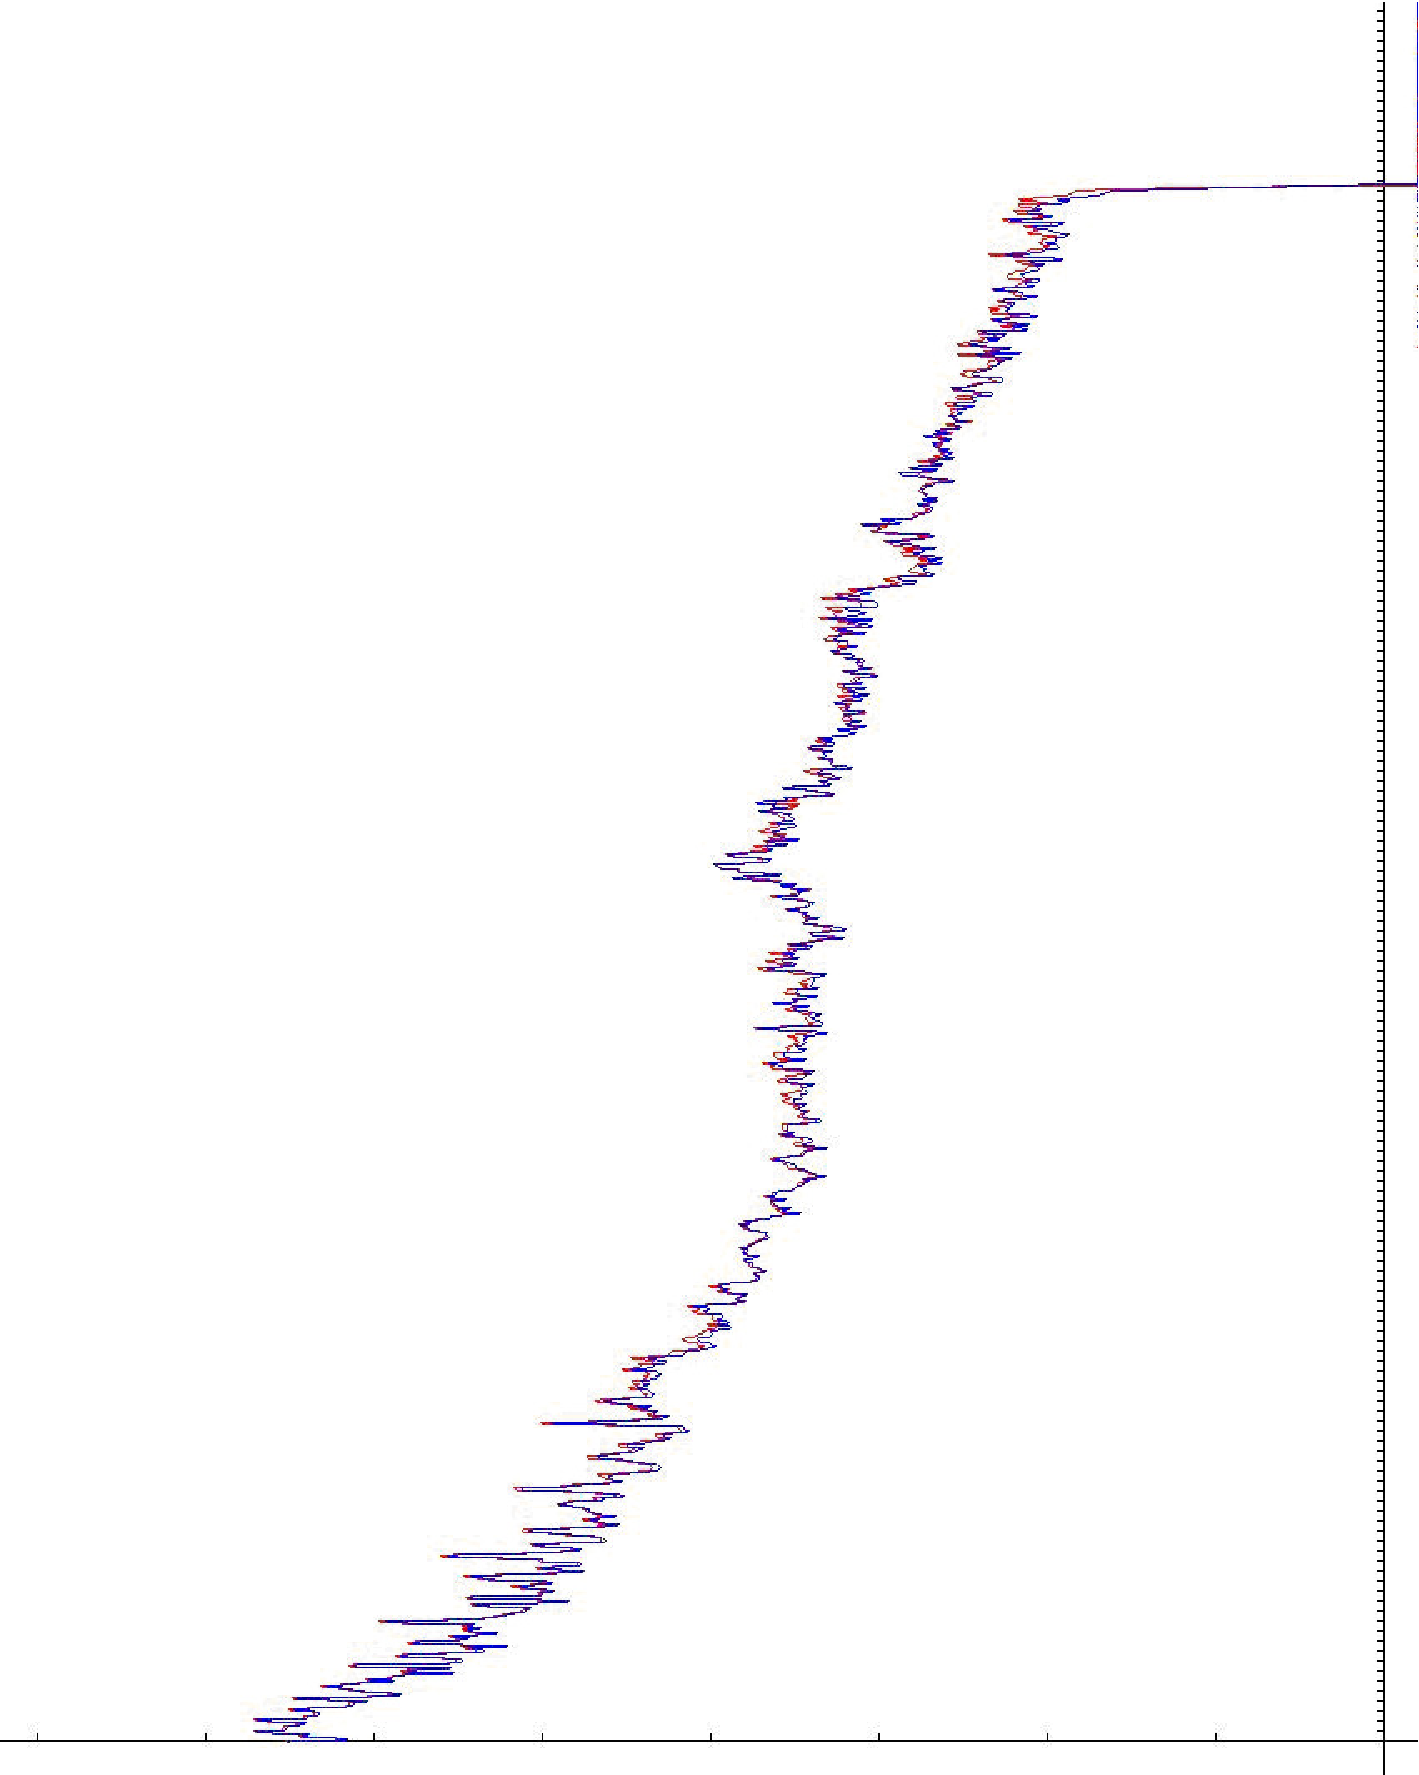
\includegraphics[scale=0.35]{withTUNEDFFT}
% 	  \caption{The activation of TUNED\_FFT does not seem to have impact on the frequency response\label{withTUNEDFFT}}
%   \end{center}
% \end{figure}
%------------------ End of figure ----------------------------------

%----------------------------------------------------------------------
\section{Test Signals}
%----------------------------------------------------------------------
\subsection{Narrow band and wideband}
For narrow band and wideband signals, ITU-T SG 12 has been
recommending input signal as Rec. ITU-T \textbf{P.50 test signals}
(p50\_m.16p for male voices, and p50\_f.16p for female voices). Those
signal are meant to be representative of speech signals.

\subsection{Superwideband and fullband}
For audio bandwidths greater than wideband, the Rec. ITU-T
\textbf{P.50 test signals} does not cover enough frequency range for
characterizing superwideband or fullband systems.

Therefore, ITU-T
SG12 has been suggesting use of Composite Source (CS) Signal as
defined in Rec.~ITU-T~P.501 as it provides sufficient energy in the
frequency range above 8~kHz and below 100~Hz. As audio coding systems
must also be capable of transmitting signals other than speech, ITU-T
SG12 has provided the following guidelines (more details are given in
\cite{AC-0801-Q10-04}):
\begin{enumerate}
\item In case CS-signal cannot be used, it is recommended to use
  artificial voice according to ITU-T Rec. P.50 and mix it with a
  broadband pink noise signal. The mixing should be 50\%/50\% ... If
  the decoded signal does not sound distorted, it can be used as an
  input test signal.

\item If the signal sounds distorted replace the artificial voice
  signal by a voice signal consisting of speech sentences (2
  sentences, 2 male, 2 female talkers each), such as ones in
  Rec. ITU-T P.501.

\item If this does not lead to the desired result replace the pink
  noise by a broadband background noise signal providing as much
  energy as possible in the high frequency range, such as ones in
  Rec. ITU-T P.501 or ETSI EG 202 396-1.

\item Codecs intended to transmit music could be tested with a
  fullband music signal. Again care should be taken to provide
  sufficient energy in the high and low frequency range.
\end{enumerate}


%----------------------------------------------------------------------
\section{Implementation}
%----------------------------------------------------------------------

%-.-.-.-.-.-.-.-.-.-.-.-.-.-.-.-.-.-.-.-.-.-.-.-.-.-.-.-.-.-.-.-.-.-.-.
\subsection{\tt rdft}

{\bf Syntax: }

{\tt
\#include "fft.h"\\
void rdft \ttpbox{110mm}{(int {\em NFFT}, float* {\em x1}, float*
{\em x2}, float* {\em y2}); }}

{\bf Prototype: }    fft.h

{\bf Description: }

This routine computes the positive part of the spectrum, using
Real Discrete Fourier Transform.

{\bf Variables: }
\begin{Descr}{\DescrLen}
\item[\pbox{20mm}{\em NFFT}] %%\rulex{1mm}\\
        number of coefficients of the Fourier transform;

\item[\pbox{20mm}{\em x1}] %%\rulex{1mm}\\
        input real signal;

\item[\pbox{20mm}{\em x2}] %%\rulex{1mm}\\
        output real part of the Fourier Transform;

\item[\pbox{20mm}{\em y2}] %%\rulex{1mm}\\
        output imaginary part of the Fourier Transform;
\end{Descr}


%-.-.-.-.-.-.-.-.-.-.-.-.-.-.-.-.-.-.-.-.-.-.-.-.-.-.-.-.-.-.-.-.-.-.-.
\subsection{\tt genHanning}

{\bf Syntax: }

{\tt
\#include "fft.h"\\
void genHanning \ttpbox{110mm}{(int {\em n}, float* {\em
hanning}); }}

{\bf Prototype: }    fft.h

{\bf Description: }

This routine generates a hanning window.

{\bf Variables: }
\begin{Descr}{\DescrLen}
\item[\pbox{20mm}{\em n}] %%\rulex{1mm}\\
        number of coefficients of the hanning window;

\item[\pbox{20mm}{\em hanning}] %%\rulex{1mm}\\
        buffer containing the coefficients of the hanning window;
\end{Descr}

%-.-.-.-.-.-.-.-.-.-.-.-.-.-.-.-.-.-.-.-.-.-.-.-.-.-.-.-.-.-.-.-.-.-.-.
\subsection{\tt powSpect}

{\bf Syntax: }

{\tt
\#include "fft.h"\\
void powSpect \ttpbox{110mm}{(float* {\em real}, float* {\em
imag}, float* {\em pws}, int {\em n}); }}

{\bf Prototype: }    fft.h

{\bf Description: }

% This routine computes the power spectrum of the DFT of a signal.
This routine computes the power spectrum of a signal with the fast
split radix DFT.

{\bf Variables: }
\begin{Descr}{\DescrLen}
\item[\pbox{20mm}{\em real}] %%\rulex{1mm}\\
        input buffer containing the real part of the DFT;

\item[\pbox{20mm}{\em imag}] %%\rulex{1mm}\\
        input buffer containing the imaginary part of the DFT;

\item[\pbox{20mm}{\em pws}] %%\rulex{1mm}\\
        output buffer containing the power spectrum;

\item[\pbox{20mm}{\em n}] %%\rulex{1mm}\\
        length of the input buffers;
\end{Descr}

%-.-.-.-.-.-.-.-.-.-.-.-.-.-.-.-.-.-.-.-.-.-.-.-.-.-.-.-.-.-.-.-.-.-.-.
\subsection{\tt actrdft}

{\bf Syntax: }

{\tt
\#include "fft.h"\\
void actrdft \ttpbox{110mm}{(int {\em n}, int {\em isgn}, float* {\em
a}, int* {\em ip}, float* {\em w}); }}

{\bf Prototype: } fft.h

{\bf Description: }

This routine computes actual fast discrete Fourier transform for real
sequence. This routine replaces ``rdft'' defined above (newly
introduced at STL2009 release).

{\bf Variables: }
\begin{Descr}{\DescrLen}
\item[\pbox{25mm}{\em n}] %%\rulex{1mm}\\
        data length, must be n $\geq$ 2 and power of 2

\item[\pbox{25mm}{\em isgn}] %%\rulex{1mm}\\
        Transform type (1 represents forward transform, -1 represents inverse)

\item[\pbox{25mm}{\em a[0...n-1]}] %%\rulex{1mm}\\
        input/output data

\item[\pbox{25mm}{\em ip[0 ... *]}] %%\rulex{1mm}\\
        work area for bit reversal

\item[\pbox{25mm}{\em w[0 ...n/2-1]}] %%\rulex{1mm}\\
        cos/sin table
\end{Descr}

%-.-.-.-.-.-.-.-.-.-.-.-.-.-.-.-.-.-.-.-.-.-.-.-.-.-.-.-.-.-.-.-.-.-.-.
\subsection{Tests and portability}

Compiled and tested on a PC (Windows) platform with MS Visual C++
6.0.

%----------------------------------------------------------------------
\section{Example code}
%----------------------------------------------------------------------

A demonstration program, {\em freqresp.c} illustrates the use of
this module to compute the average power spectrum of two signals
(input and output of the codec).

The syntax needed for using the variable size is following:
{\tt\small
\begin{verbatim}
  freqresp.exe -nfft 4096 FileInpCodec FileOutCodec ASCIIout}
\end{verbatim}}
If the {\tt -nfft} option is not used, then the default size (2048) is used. The other usual options (e.g. sampling frequency,\ldots) can still be set.

The max length of FFT is defined by the macro "{\tt NFFT\_MAX}" and is set to 8192. 

